\documentclass[conference]{IEEEtran}

\hyphenation{op-tical net-works semi-conduc-tor}

\usepackage{amsmath}
\usepackage{amssymb}
\usepackage{amsthm}
\usepackage{graphicx}
\usepackage{hyperref}

\newtheorem{mydef}{Definition}
\newtheorem{mylem}{Lemma}
\newtheorem{mythm}{Theorem}
\newtheorem{myprop}{Property}
\newtheorem{mycoro}{Corollary}


\begin{document}

\title{Input-to-state stable analysis on Particle Swarm Optimization}

\author{
\IEEEauthorblockN{Daqing Yi,
Kevin D. Seppi, and Michael A. Goodrich}

\IEEEauthorblockA{Department of computer science, Brigham Young University, Provo, UT 84604 USA}
\thanks{}
}

% The paper headers
%\markboth{Journal of \LaTeX\ Class Files,~Vol.~11, No.~4, December~2012}%
%{Shell \MakeLowercase{\textit{et al.}}: Bare Demo of IEEEtran.cls for Journals}
\markboth{}{}

\maketitle

\begin{abstract}
This paper examines the dynamics of particle swarm optimization (PSO) by modeling PSO as a cascade system and then applying input-to-state stability analysis.
Using a cascade system model we can
include the effects of the global-best and personal-best values more directly in the model of the dynamics.
Thus in contrast to previous study of PSO dynamics, the input-to-state stability property used here allows for the analysis of PSO both before and at stagnation.
In addition, the use of input-to-state stability allows this analysis to preserve random terms which were heretofore simplified to constants.
This analysis is important because it can inform the setting of PSO parameters and better characterize the nature of PSO as a dynamic system.
This work also illuminates the way in which the personal best and the global best updates influence the bound on particle's position and hence, how the algorithm
exploits and explores the fitness landscape as a function of the personal best and global best.
\end{abstract}

\begin{IEEEkeywords}
Particle swarm optimization, input-to-state stability
\end{IEEEkeywords}

\IEEEpeerreviewmaketitle

\section{Introduction}
\label{sec:intro}

This project is based on ``Distributed cooperative attitude synchronization and tracking for multiple rigid bodies'' by Dr. Ren \cite{5229134}, in which discusses the consensus seeking of a system of agents with non-linear model.
Two approaches have been proposed for ``cooperative attitude synchronization'' (position control) and ``reference attitude tracking'' (trajectory tracking) respectively.
Two approaches are stated independently and look different.
One objective of this project is seeking the consensus between two approaches, which can be used as a pattern on analyzing other synchronization systems and designing control laws for them.

The structure of this report is as following.
Section \ref{sec:prob_stat} states the system model, which includes the rigid body dynamics of each agent and the interaction topology.
Section \ref{sec:coop_att_syn} presents the control law proposed for the cooperative attitude synchronization and the proof strategy.
%I try to figure out the roles of the terms in the control law so that I can simplify the control law with ignorance on the transient performance and prove the stability.
By analyzing the roles of the terms in the control law, I simplify the control law to find the essential component that guarantees the stability.
It means that the stability can still be preserved and proved without some terms for transient performance.
Section \ref{sec:ref_att_trk} illustrates the control law proposed for the reference attitude tracking and the proof strategy.
I use a same proof strategy to prove the stability of the control law on the cooperative attitude synchronization, which shows the consistency between two approaches.
It means that the ideas of improvement can be applied to both control approaches.
Simulations are also taken on both approaches for analysis purpose.
Section \ref{sec:io_stable} proposes an interconnection perspective for analyzing a class of distributed system control problems as a pattern of analyzing a consensus-seeking problem.
A hypothesis on proving the stability is proposed, in which the proof can be achieved by analyzing the stability-relevant properties of the sub-components.
Section \ref{sec:summary} discusses some possible future work from Dr. Ren's paper.

\section{Related Work}
\label{sec:related_work}

If we assume that search targets are static in the search environment, the scan on a location decreases the estimated probability that there is some search target here.
Observations in a search process reduce the uncertainty of where search targets locate.
By measuring this type of uncertainty with information, a search agent can collect more information at non-observed locations than observed ones.
Information gathering is usually selected to measure the efficiency of a search task.
In this paper, we focus on path planning in a search task answers how to maximize information with limited time and resource by defining objective in forms of information evaluation \cite{goodrich2013toward}.

Research work on information maximization path planning focuses a lot on how to solve the optimization problems defined in large scale solution spaces in reasonable time.
\cite{levine2010information} imports ideas of RRT to an information-rich path planning problem, which targets at bringing good efficiency in online optimization in a continuous space.
Under a temporal logic constraint, \cite{JonesSchwagerBeltaICRA13scLTLInfo} use a receding horizon planning to solve an online information-gathering optimization problem.

\begin{figure}
\centering
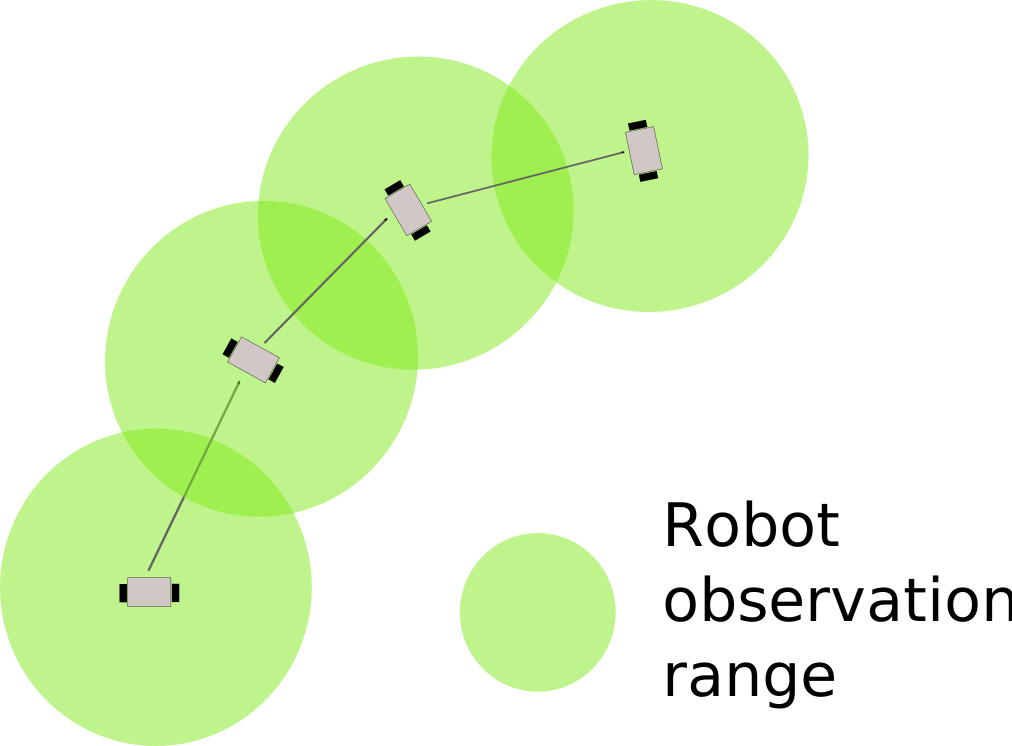
\includegraphics[width=0.4\linewidth]{./images/robotObservation.pdf}
\caption{Maximum coverage in robot observation.}
\label{fig:robotObservation}
\end{figure}

Usually the observation of a search agent covers a much larger region than the area occupied by the robot's body, which is shown in Figure \ref{fig:robotObservation}.
If we consider the observation as a covering range instead of a cell or a point, the overlaps between observation coverage at different time steps must be considered when measuring the total quantity of information.
Figure \ref{fig:robotObservation} gives an example.

Mutual information and conditional mutual information are commonly used to model the overlaps in measuring the total information \cite{singh2009efficient}.
This belongs to a \emph{maximum coverage problem}. 
Multiple sensors placement is one of the applications on information maximization.
In a sequential placement, the locations of placed sensors determine the increase on total information by adding a new sensor.
It is known to be a classical NP-hard combinatorial optimization problem \cite{megiddo1983maximum}.
The problem of maximum coverage on information measurement implies a property of ``nondecreasing submodularity''. 

Maximizing the score collected from a limited-length graph walk is usually known as an \emph{orienteering problem} \cite{Vansteenwegen20111}, in which the total score is a summation of the scores of visited vertices.
If the score function of a vertex has submodularity as in a \emph{maximum coverage problem}, the problem is defined as a \emph{submodular orienteering problem} \cite{chekuri2005recursive}.
A greedy approximation with known performance bound proposed in \cite{singh2009efficient} efficiently exploits the submodularity property of mutual information.
Similarly, in a branch and bound way, \cite{binney2012branch} apply greedy search to informative path planning.
Because the location of the robot at time $ t $ constrains the reachable location at time $ t+1 $, applying greedy algorithm with ``teleport'' assumption to the problem with this constraint can be extremely bad \cite{krause2012submodular}.
In non-teleport motion, \cite{chekuri2005recursive} import recursive greedy by converting to a knapsack constraint so that there is a time resource allocation on planning steps.

Due to the wingman constraint, the path planning of a robot wingman depends on a temporal-space synchronization requirement determined by the positions of a human through time.
The time allocation is fixed and depends on how the human's positions are sampled.
Thus we are not able to model time resource as budget in \cite{chekuri2005recursive}.   

We define the path planning of the robot wingman in a search task as an information maximization problem on a topological graph. We propose an algorithm to solve it as submodular orienteering . The algorithm is designed to produce acceptable robot performance and to be computed efficiently. We then use simulation to demonstrate the acceptable performance of the algorithm and computation efficiency. 


\section{A Cascade Model of Standard PSO}
\label{sec:sys_model}

In this paper, we model the behavior of the PSO algorithm as a \emph{cascade system}.
This enables analysis of PSO with stochastic factors preserved and without the stagnation assumption.
As shown in Figure \ref{fig:sys_flow}, this system is comprised of two components that form a
cascade system structure.
These two components are the 
\emph{input update component} for the global best ($ x^{G}_{i}(k) $) and the personal best ($ x^{P}_{i}(k) $), and the 
\emph{position update component} for particle position ($ x_{i}(k+1) $), which depends on the inputs $ x^{G}_{i}(k) $ and $ x^{P}_{i}(k) $ as well as the last position $ x_{i}(k) $ and the swarm topology.

\begin{figure}
\centering
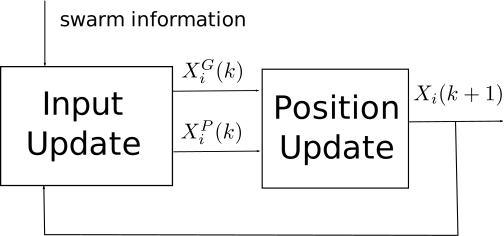
\includegraphics[width=0.5\textwidth]{sys_flow.pdf}
\caption{System structure of PSO}
\label{fig:sys_flow}
\end{figure}

The properties of this system can be analyzed using the input-to-state stability of the position update component and the input update component. 
Given an input-to-state stable position update component, we will see that the convergence of $ x_{i}(k) $ depends on bounds on $ x^{G}_{i}(k) $ and $ x^{P}_{i}(k) $.

%PSO is designed to strike an effective balance between \emph{exploring} and \emph{exploiting} a fitness landscape.
%A bound on a particle's state is an indicator of the nature of that balance.
%When this bound is large the particle is exploring.
%However, as a particle finishes exploring and reach stagnation, a particle's position should converge.
%
%Input-to-state stability implies that the state of the system is bounded in a range determined by the bounds on the input.
%Before stagnation, when the personal best and global best values have not converged, we can expect only looser bounds on the particle state.
%These looser bounds reflect both what is know about the input and the what is know about the update process itself.
%
%
%We call the bounds on the global best and personal best the ``exploit radius'' and the bounds on the particle's position a ``explore radius''.
%The ratio of the explore radius to the exploit radius is determined by the parameters of the position update component.
%However, if the personal best and global best converge to an estimated optimal position, the exploit radius falls to zero and the explore radius declines to a bound.
%
%\begin{figure}
%\centering
%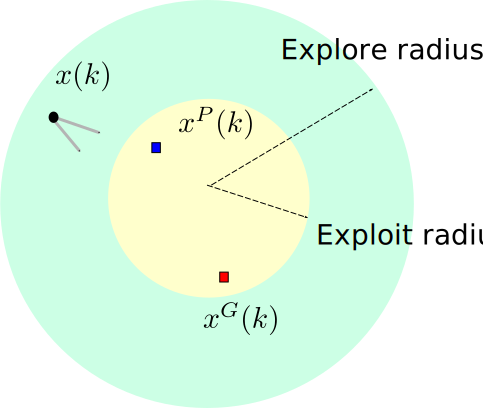
\includegraphics[width=0.4\textwidth]{./explore_and_exploit}
%\caption{Exploration and exploitation.}
%\label{fig:explore_and_exploit}
%\end{figure}

In our analysis of the PSO algorithm, we seek to understand how the particles converge to some position $ x^{*} $, which is intended (not guaranteed) by the algorithm to be the optimal position.

Without loss of generality, we look at a one-dimension particle and extract the linear form of the position update component.
\begin{equation}
\label{eq:pso_up_linalg_simp}
X(k+1) = A(k) X(k) + B(k) U(k)
\end{equation}
with
$ A(k) = \begin{bmatrix}
\chi & - \chi \phi^{G} u^{G}(k) - \chi \phi^{P} u^{P}(k)
\\ 
\chi & 1 - \chi \phi^{G} u^{G}(k) - \chi \phi^{P} u^{P}(k)
\end{bmatrix} $
and
$ B(k) = \begin{bmatrix}
\chi \phi^{G} u^{G}(k) & \chi \phi^{P} u^{P}(k)
\\ 
\chi \phi^{G} u^{G}(k) & \chi \phi^{P} u^{P}(k)
\end{bmatrix} $.

The system state is $ X(k) = [ v(k), x(k) - x^{*} ]^{T} $, and the system input is $ U(k) = [ x^{G}(k) - x^{*} , x^{P}(k) - x^{*} ]^{T} $
\footnote{$ x^{*} $ means an equilibrium point to the system.
In PSO, it can be a local optimum, a global optimum, or an estimated optimum.
We use it as a reference point to check the bounds.}
.
The convergence of this model means that $ v(k) \rightarrow 0 $ and $ x(k) \rightarrow x^{*} $.



\section{Input-to-state stability}
\label{sec:iss}

%\begin{itemize}
%\item ISS of a particle (use an appendix if long)
%\item Parameters need for a particle to be ISS
%\item Contrast with the empirical approach of Clerc and Kennedy??
%\item Use appendix for mean and variance analysis
%\end{itemize}

The properties of this system can be analyzed using the input-to-state stability of the position update component. 
Given an input-to-state stable position update component, we will see that the convergence of $ x_{i}(k) $ depends on bounds on $ x^{G}_{i}(k) $ and $ x^{P}_{i}(k) $.

Without loss of generality, we look at a one-dimension particle.
The parallel connection of input-to-state stable components reserves the input-to-state stability.

In our analysis of the PSO algorithm, we seek to understand how the particles converge to some position $ x^{*} $, which is intended (not guaranteed) by the algorithm to be the optimal position.
The convergence of this model means that $ v(k) \rightarrow 0 $ and $ x(k) \rightarrow x^{*} $.

\subsection{Input-to-state stability of the position update}

In this section, we briefly review the definition of input-to-state stability (ISS) including both the conditions that guarantee it and the bound that ISS implies\cite{Jiang2001857}. 
We then show that PSO satisfies this definition when the parameters of PSO are set in the requisite range.
We also derive the bounds implied by the ISS property.
We use the ISS property to find bounds on particle motion.

We first introduce several types of functions \cite{Jiang2001857}.
\begin{itemize}
\item $ K $-function $ \mathbb{K} $ : a function $ \alpha  : [ 0, a ) \rightarrow [ 0, \infty ) $ is continuous, strictly increasing and $ \alpha (0) = 0 $; it is a $ K_{\infty} $-function, if $ \alpha (s) \rightarrow \infty $ as $ s \rightarrow \infty $;
\item $ KL $-function $ \mathbb{KL} $ : a function $ \beta : [ 0, a ) \times [ 0 , \infty ) \rightarrow [ 0, \infty ) $ satisfies:
\begin{enumerate}
\item $ \forall t \geq 0 $, $ \beta (\cdot , t ) $ is a $ K $-function;
\item $ \forall s \geq 0 $, $ \beta (s, \cdot) $ is decreasing and $ \beta(s,t) \rightarrow 0 $ as $ t \rightarrow \infty $.
\end{enumerate}
%\item Positive-definite function: a function $ \gamma (s) > 0, \forall s > 0 $ and $ \gamma (0) = 0 $.
\item ISS-Lyapunov function $ V : \mathbb{R}^{n} \rightarrow \mathbb{R}_{\geq 0} $ satisfies:
\begin{enumerate}
\item $ \exists \alpha_{1}, \alpha_{2} \in \mathbb{K} $ such that 
$ \forall \xi \in \mathbb{R}^{n}, \alpha_{1} ( | \xi | ) \leq V( \xi ) \leq \alpha_{2}  ( | \xi | ) $.
\item $ \exists \alpha_{3} \in \mathbb{K}_{\infty} , \sigma \in \mathbb{K} $ such that $ \forall \xi \in \mathbb{R}^{n}, \forall \mu \in \mathbb{R}^{m}, V( f( \xi, \mu ) ) - V( \xi ) \leq - \alpha_{3} ( | \xi | ) + \sigma ( | \mu | ) $. 
\end{enumerate}
\end{itemize}

\begin{mydef}[Input-to-state stable]\cite{Jiang2001857}
\label{def:iss}
For a discrete-time system
\begin{equation}
\label{eq:dis_nonlinear}
x(k+1) = f( x(k) , u(k) ),
\end{equation}
with $ f(0,0) = 0 $
\footnote{This means that $ x = 0 $ is an equilibrium of the 0-input system.}, the system is \emph{(globally) input-to-state stable} if there exist a $ KL $-function $ \beta  $ and a $ K $-function $ \gamma $ such that, for each input $ u \in l^{m}_{\infty} $ and each $ \xi \in \mathbb{R}^{n} $, it holds that $  \forall k \in \mathbb{Z}^{+} $,
\begin{equation}
\label{eq:def_iss}
| x(k, \xi, u) | \leq \beta (| \xi |, k) + \gamma ( \lVert u \rVert ).
\end{equation}
\end{mydef}

The $ \beta () $ term in \eqref{eq:def_iss} defines an initial bound with a decaying property.
The $ \gamma () $ term in \eqref{eq:def_iss} defines a bound determined by the input.
This means that the influence $ \beta () $ term gradually decreases to zero and the position is bounded by a range determined by the bound on the input.
An ISS-Lyapunov function, defined above, can be used to prove the input-to-state stability of a system and analyze the state bound\cite{Jiang2001857}.
We will use the ISS-Lyapunov-function approach in the proof given later in this section.

\subsection{Conditions for input-to-state stability for position update in PSO}

Using the definition of the PSO position update as given in \eqref{eq:pso_up_linalg_simp}, PSO can be shown to be ISS as defined in definition \ref{def:iss}.

\begin{mythm}
\label{thm:iss}
The system \eqref{eq:pso_up_linalg_simp} is input-to-state stable, when $ | \lambda_{\max} ( A(k) ) | < 1 $.
%The system \eqref{eq:pso_up_linalg_simp} is input-to-state stable, if there exists a symmetric positive definite matrix $ P $ and a symmetric positive definite matrix $ Q' $ that has $ A(k)^{T} P A(k) - P = - Q(k) \leq - Q' $.
\begin{proof}

Let $ P $ be an identity matrix.
As $ | \lambda_{\max} ( A(k) ) | < 1 $, we have
$ \lVert A^{T}(k) P A(k) \rVert \leq \lVert P \rVert \lVert A(k) \rVert^{2} \leq \lVert P \rVert | \lambda_{\max} ( A(k) ) |^{2} < \lVert P \rVert $.
Because $ P $ is an identity matrix it is positive definite, and thus $ A^{T}(k) P A(k) $ is positive definite or positive semi-definite by definition.
So by positive definite ordering we have $ A^{T}(k) P A(k) < P $.

Let $ -Q(k) = A^{T}(k) P A(k) - P $. Since $ A^{T}(k) P A(k) < P $ then $ - Q(k) < 0 $ furthermore $ \exists Q' \forall k, Q(k) > Q' > 0 $. 

By the Lemma 3.5 in \cite{Jiang2001857}, if we can show that a proposed positive definite Lyapunov function is an ISS-Lyapunov function, then the system is ISS.

Define a Lyapunov function
\begin{equation}
\label{eq:lyapunov_v}
V( X(k) ) = X^{T} (k) P X(k).
\end{equation}
We can have
$
\lambda_{min}(P) | X(k) |^{2} \leq V( X(k) )\leq \lambda_{max}(P) | X(k) |^{2}
$ and $ \lambda_{min}(P) = \lambda_{max}(P) $.

Let $ \alpha_{1} ( \xi )= \lambda_{min} \xi^{2} $
and 
$ \alpha_{2} ( \xi )= \lambda_{max} \xi^{2} $,
we have $ V(x) $ satisfying condition 1 of the ISS-Lyapunov function definition.

By applying \eqref{eq:pso_up_linalg_simp} to $ V( X(k+1) ) - V( X(k) ) $, we have
\begin{equation}
\label{eq:lyapunov_delta2}
\begin{aligned}
& V( X(k+1) ) - V( X(k) ) \\
= & - X^{T}(k) [ A^{T}(k) P A(k) - P ] X(k)  \\
& + 2 X^{T}(k)  A^{T}(k) P B(k) U(k) + U^{T}(k) B^{T}(k) P B(k) U(k) \\
\leq & - X^{T}(k) Q' X(k) + 2 X^{T}(k)  A^{T}(k) P B(k) U(k) \\
& + U^{T}(k) B^{T}(k) P B(k) U(k) \\
\leq & - \lambda_{min}(Q') | X(k) |^{2} + 2  \lVert A^{T}(k) P B(k) \rVert | U(k) | | X(k) | \\
& + \lVert B^{T}(k) P B(k) \rVert | U(k) |^{2}.
\end{aligned}
\end{equation}

By completing the square, we have
\begin{equation}
\label{eq:lyapunov_delta4}
\begin{aligned}
& V( X(k+1) ) - V( X(k) ) \\
\leq & - \frac{1}{2} \lambda_{min}(Q') | X(k) |^{2} + [ \frac{2 \lVert A^{T}(k) P B(k) \rVert^{2}}{ ( \lambda_{min}(Q') )^{2} }  \\
& + \lVert B^{T}(k) P B(k) \rVert ] | U(k) |^{2}. 
\end{aligned}
\end{equation}

Because $ u^{P}(k) \in [0, 1] $, there exist an $ A' $ and $ B' $ such that $ \lVert A(k) \rVert \leq \lVert A' \rVert $ and $ \lVert B(k) \rVert \leq \lVert B' \rVert $.
We have $ \lVert A^{T}(k) P B(k) \rVert \leq \lVert A' \rVert \lVert P \rVert \lVert B' \rVert $ and $ \lVert B^{T}(k) P B(k) \rVert \leq \lVert P \rVert \lVert B' \rVert^{2} $.

Since the identity matrix $ P $ has $ || P || = 1 $:
\begin{equation}
\label{eq:lyapunov_delta5}
\begin{aligned}
& V( X(k+1) ) - V( X(k) ) \\
\leq & - \frac{1}{2} \lambda_{min}(Q') | X(k) |^{2} + [ \frac{2 \lVert A' \rVert^{2} \lVert B' \rVert^{2}}{ ( \lambda_{min}(Q') )^{2} } + \lVert B' \rVert^{2} ] \lVert U(k) \rVert^{2}.
\end{aligned}
\end{equation}

Let
$ \alpha_{3} ( \xi )= \frac{1}{2} \lambda_{min}(Q') \xi^{2} $,
and
$ \sigma ( \xi ) = [ \frac{2 \lVert A' \rVert^{2} \lVert B' \rVert^{2}}{ ( \lambda_{min}(Q') )^{2} } +  \lVert B' \rVert^{2} ] \xi^{2} $.
Thus we have $  V( X(k+1) ) - V( X(k) ) $ satisfying condition 2 of the ISS-Lyapunov function definition and
so \eqref{eq:lyapunov_v} is an ISS-Lyapunov function.
Using Lemma 3.5 in \cite{Jiang2001857}, the position update component of PSO \eqref{eq:pso_up_linalg_simp} is input-to-state stable.

\end{proof}
\end{mythm}

Note that in using \eqref{eq:pso_up_linalg_simp} with $ x^{R} = x^{*} $,
$ [ v(k), x(k) - x^{*} ]^{T} = [0, 0]^{T} $ is an equilibrium position when the input $ [ x^{G}(k) - x^{*} , x^{P}(k) - x^{*} ]^{T} = [0, 0]^{T} $.
For an arbitrary optimization problem $ x^{R} $ would typically not be at the origin. 
In such a problem, input-to-state stability means that the boundaries of $ \lVert v(k) \lVert $ and $ \lVert x(k) - x^{R} \rVert $ would be transformed and thus determined by $ | x^{G}(k) - x^{R} | $ and $ | x^{P}(k) - x^{R} | $,
but the properties of ISS still apply independent of where the function is centered.
Having proven that PSO is ISS we can now state a bound on particle position.

\begin{mythm}
\label{thm:state_bound}
Given the bound on the input $ \lVert u \rVert $ in the position update component, we have the bound on the particle position from \eqref{eq:pso_up_linalg_simp}.
\begin{equation}
\label{eq:state_bound}
\forall k, 
| x(k+1) - x^{R} | \leq \max ( | x(0) - x^{R} | , \gamma ( | [ x^{G}(k) - x^{R}, x^{P}(k) - x^{R} ]^{T} | ) ),
\end{equation}
in which $ \gamma = \alpha_{3}^{-1} \circ \sigma $.

The $ \max $ part is needed to account for the effect of the starting point, represented by the first parameter. Eventually the effect of the starting point no longer affects the system, formally:
\begin{equation}
\label{eq:state_bound:conv}
\exists T, \forall k \geq T, 
|  x(k+1) - x^{R} | \leq \gamma ( | [ x^{G}(k) - x^{R}, x^{P}(k) - x^{R} ]^{T} | ).
\end{equation}
\begin{proof}
As we have the update equation as
$ X(k+1) = A(k) X(k) + B(k) U(k) $, we can derive 
\begin{equation}
X(k+1) = ( \prod_{k}^{i=0} A(i) ) X(0) + \sum_{i=0}^{k} [ ( \prod_{j=0}^{i-1} A(j) ) B(i) U(i)  ] 
\end{equation}
by recursively applying it.

By the property of matrix norm, we have
\begin{equation}
| X(k+1) | \leq ( \prod_{i=0}^{k} \lVert A(i) \rVert ) | X(0) | + \sum_{i=0}^{k} [ ( \prod_{j=0}^{i-1} \lVert A(j) \rVert ) \lVert B(i) \rVert | U(i) |  ].
\end{equation}

$ \forall i \in [0, k] $, let $ \lVert A(i) \rVert \leq \lVert A \rVert $, $  \lVert B(i) \rVert \leq \lVert B \rVert $ and $ | U(k) | = [ x^{G}(k) - x^{R}, x^{P}(k) - x^{R} ]^{T} $, we have
\begin{equation}
\label{eq:bound:final}
\begin{aligned}
& |  x(k+1) - x^{R} | \leq | X(k+1) | \\
& \leq ( \lVert A \rVert )^{k+1} | X(0) | + \sum_{i=0}^{k} [ ( \lVert A \rVert )^{i} \lVert B \rVert | U(i) |  ] \\
& = ( \lVert A \rVert )^{k+1} | X(0) | + \frac{1 - ( \lVert A \rVert )^{k+1} }{1 - \lVert A \rVert }  \lVert B \rVert | U(i) |
\end{aligned}
\end{equation}

%The boundary will be a function of $ bound ( \lVert A \rVert, \lVert B \rVert, | X(0) |, | U |, k ) $.
%Thus the minimum boundary is $ \min_{k} bound ( \lVert A \rVert, \lVert B \rVert, | X(0) |, | U |, k ) $.
%When we have $ \lVert A \rVert < 1 $, 
%$ ( \lVert A \rVert )^{k+1} \rightarrow 0 $ and
%$ \frac{1 - (\lVert A \rVert )^{k+1} }{1 - \lVert A \rVert} \rightarrow \frac{1}{1 - \lVert A \rVert } $
%as $ k \rightarrow \infty $.

$ ( \lVert A \rVert )^{k+1} $ shows the decay term and $ \frac{1 - ( \lVert A \rVert )^{k+1} }{1 - \lVert A \rVert }  \lVert B \rVert $ makes the boundary function $ \gamma () $.

\end{proof}
\end{mythm}

Figure \ref{fig:boundary} gives an example on how a particle's boundary is determined by the personal best and global best.

\begin{figure}
\centering
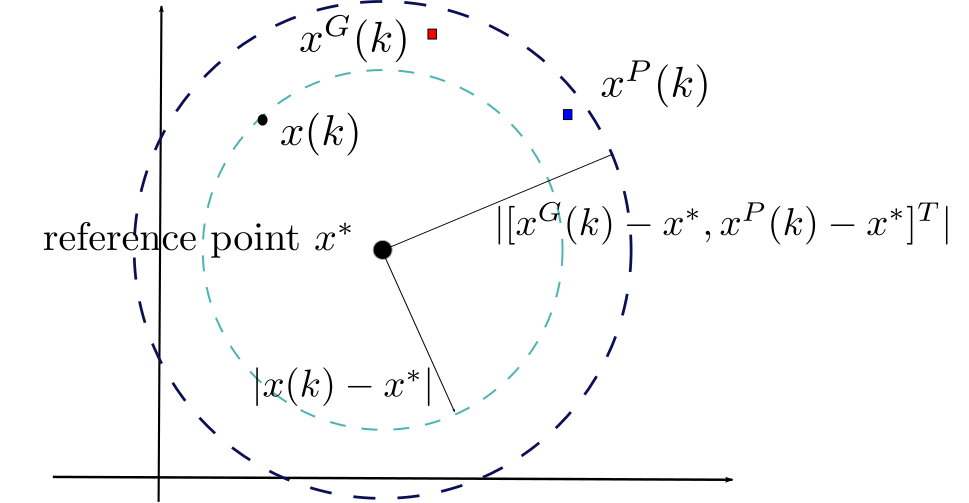
\includegraphics[width=0.6\linewidth]{./fig/boundary}
\caption{A bound on a particle's position by a reference point $ x^{*} $ from Equation \ref{eq:state_bound:conv}.
The ratio of wo radii indicates $ \gamma $.}
\label{fig:boundary}
\end{figure}

\begin{mycoro}
\label{coro:param_unit_disc}
Write $ A(k) = 
\begin{bmatrix}
\chi & - \chi \phi \\
\chi & 1 - \chi \phi
\end{bmatrix}
$, in which
$ \phi \in [0,  \phi^{P} + \phi^{G} ] $ and $ \chi \in ( 0, 1 ) $.
When $ \phi \in (0 , \frac{2(1+\chi)}{\chi} ) $, the system \eqref{eq:pso_up_linalg_simp} is input-to-state stable.
\begin{proof}
Let $ a = (1 + \chi) - \chi \phi $. 
The eigenvalues of $ A(k) $ are
$ \lambda = \frac{ a \pm \sqrt{ a^{2} - 4 \chi } }{2} $.

\begin{enumerate}
\item If $ a^{2} \geq 4 \chi $, we have $ a \geq 2 \sqrt{\chi} $ or $ a \leq - 2 \sqrt{\chi} $.

If $ a \geq 2 \sqrt{\chi} $, then $ | \lambda_{\max} | < 1 $ derives $ 0 < \frac{a-\sqrt{a^{2}-4\chi}}{2} \leq \frac{a+\sqrt{a^{2}-4\chi}}{2} < 1 $.
It means that $ 2 \sqrt{ \chi } \leq a < 1 + \chi $.

If $ a \leq 2 \sqrt{\chi} $, then $ | \lambda_{\max} | < 1 $ derives $ -1 < \frac{a-\sqrt{a^{2}-4\chi}}{2} \leq \frac{a+\sqrt{a^{2}-4\chi}}{2} < 0 $.
It means that $ - (\chi+1) < a \leq - 2 \sqrt{\chi} $.

\item If $ a^{2} \geq 4 \chi $, we have $ - 2 \sqrt{\chi} < a < 2 \sqrt{\chi} $.

$ | \lambda_{\max} | < 1 $ derives $ \frac{ a^{2} }{4} + \frac{ a^{2} - 4\chi }{4} < 1 $.
It means that $ - 2 \sqrt{ 2(1+\chi) } < a < 2 \sqrt{ 2(1+\chi) } $.
Because $ \sqrt{ 2(1+\chi) } > 2 \sqrt{ \chi } $, we have $ - 2 \sqrt{\chi} < a < 2 \sqrt{\chi} $.
\end{enumerate}
Combining these two cases, we have  $ - (1 + \chi) < a < 1 + \chi $.
It equals to $ \phi \in (0 , \frac{2(1+\chi)}{\chi} ) $.

\end{proof}
\end{mycoro}

Figure \ref{fig:paramSpace} shows the parameter space.
The x-axis is $ \phi = \phi^{P} + \phi^{G} $ and the y-axis is $ \chi $.
The stable region in red is obtained from eigenvalue test on Theorem \ref{thm:iss} and the yellow boundary is obtained from Corollary \ref{coro:param_unit_disc}.
\begin{figure}
\centering
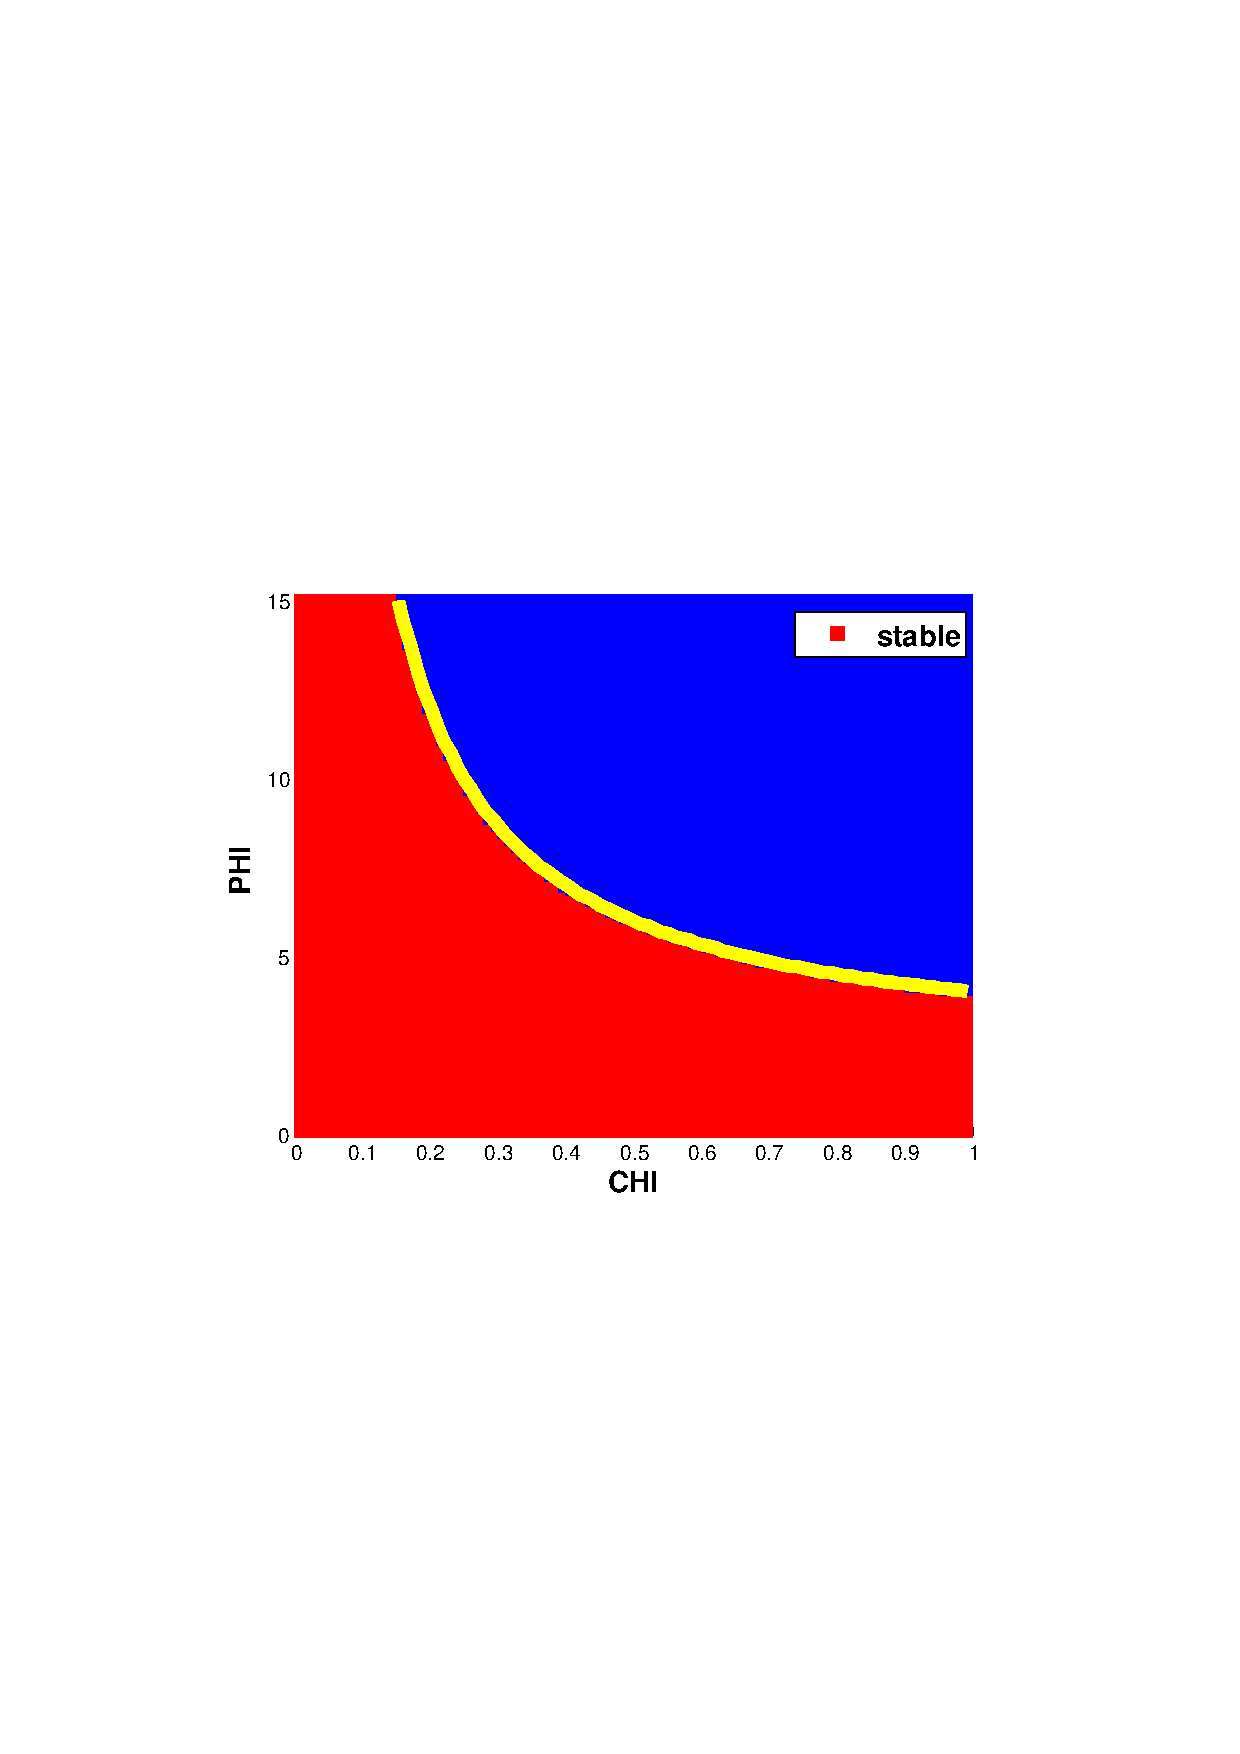
\includegraphics[width=0.5\linewidth]{./fig/param2}
\caption{Parameter space}
\label{fig:paramSpace}
\end{figure}


%Since by Theorem \ref{thm:iss} PSO is ISS, and therefore by Corollary \ref{coro:state_bound} the stability of the cascade system depends on the output of the input update component. We can say:
%\begin{enumerate}
%\item If the input update component generates converging personal best and global best, the bound of the particle position will converge;
%\item If the personal best and global best vary within a bound, the particle will converge within a bound;
%\item If the personal best and global best become constant, the particle will converge to a point.
%\end{enumerate}
%Furthermore, by equation \eqref{eq:state_bound}, we know that the convergence of a particle's position $ x(k) $ to $ x^{*} $ depends on how $ x^{P}(k) $ and $ x^{G}(k) $ converge to $ x^{*} $, if the position update component is input-to-state stable.
%In particular, the boundary of the distance between a particle's position and  $ x^{*} $ is determined by the initial distance $ x(0) -  x^{*} $, $ x^{P}(k) -  x^{*} $ and $ x^{G}(k) -  x^{*} $.

%Answer two questions here
% a) why we need iss of position update 
% b) what else do we need for iss

The input-to-state stability of the position update component makes the movement of a particle bounded in a range that covers the global best and the personal best.
This property provides the chance that the particle exploits the regions near around the personal best and the global best.
We can have:
\begin{enumerate}
\item If the personal best and global best converge, the bound of the particle position will converge;
\item If the personal best and global best vary within a bound, the particle will converge within a bound;
\item If the personal best and global best become constant, the particle will converge to a point.
\end{enumerate}
Furthermore, by \eqref{eq:state_bound}, we know that the convergence of a particle's position $ x(k) $ to $ x^{R} $ depends on how $ x^{P}(k) $ and $ x^{G}(k) $ converge to $ x^{R} $, if the position update component is input-to-state stable.
In particular, the boundary of the distance between a particle's position and  $ x^{R} $ is determined by the initial distance $ x(0) -  x^{R} $, $ x^{P}(k) -  x^{R} $ and $ x^{G}(k) -  x^{R} $.
Conversely, if the position update component is not input-to-state stable, the movement of the particle will diverge from the global best and the personal best.
The design of the exploitation by the personal best and the global best is lost.
%As in Figure \ref{fig:sys_flow}, the position update component and the input update component are serially connected.
When the position update component is input-to-state stable, the input-to-state stability of the particle is determined by the input-to-state stability of the personal best update component.
However, the input-to-state stability of the input update component depends on the fitness distribution, which could not be guaranteed in many cases.
In section \ref{sec:particle}, we will analyze the behavior of the particle when the position update component is input-to-state stable.
We will later extend the analysis to the swarm in section \ref{sec:swarm}.





\section{The Stability after including Input Update Component}
\label{sec:opt_strgy}

In this section, we add the input update component that was first shown in Figure \ref{fig:sys_flow} and then analyze the convergence of particle position.

%For a minimization problem, the standard input update component is usually written as
%\begin{equation}
%\label{eq:update_b}
% x^{P}(k) = \arg \min_{ x \in \{ x(k), x^{P}(k-1) \} } f( x )
% \; and \;
% x^{G}(k) = \arg \min_{ x \in \{ x(k), X^{G}(k) \} } f( x ),
%\end{equation}
%in which $ X^{G}(k) $ is a set that contains the $ x^{G} (k) $ of all the particles.

Since by Theorem \ref{thm:iss} PSO is ISS, and therefore by Corollary \ref{coro:state_bound} the stability of the cascade system depends on the output of the input update component. We can say:
\begin{enumerate}
\item If the input update component generates converging personal best and global best, the bound of the particle position will converge;
\item If the personal best and global best vary within a bound, the particle will converge within a bound;
\item If the personal best and global best become constant, the particle will converge to a point.
\end{enumerate}

Furthermore, by equation \eqref{eq:state_bound}, we know that the convergence of a particle's position $ x(k) $ to $ x^{*} $ depends on how $ x^{P}(k) $ and $ x^{G}(k) $ converge to $ x^{*} $, if the position update component is input-to-state stable.
In particular, the boundary of the distance between a particle's position and  $ x^{*} $ is determined by the initial distance $ x(0) -  x^{*} $, $ x^{P}(k) -  x^{*} $ and $ x^{G}(k) -  x^{*} $.

As the stagnation is defined that there is no new improvement found, we have that $ x^{P}(k) $ and $ x^{G}(k) $ are constant, which are $ x^{P} $ and $ x^{G} $ respectively.
If we assume that $ u^{P}(k) $ and $ u^{G}(k) $ are equivalent and constant, it is stated that
\begin{equation}
\label{eq:single_obj_equilibrium}
\hat{x} = \frac{\phi^{P} x^{P} + \phi^{G} x^{G} }{ \phi^{P} + \phi^{G} } 
\end{equation}
is an equilibrium point for stagnation as noted in previous work \cite{985692}.

By letting $ x^{*} = \hat{x} $ be the reference point, and
by Corollary \ref{coro:state_bound}, we can go beyond prior work and can identify a bound on PSO behavior at stagnation:
\begin{equation}
\label{eq:single_obj_input_bound}
\exists T, \forall k > T, 
| x(k) - \hat{x} | \leq  \gamma_{d} | [ x^{P} - \hat{x}, x^{G} - \hat{x} ]^{T} |,
\end{equation}
with 
\begin{equation}
 \gamma_{d} = \frac{ 2 \lVert A' \rVert^{2} \lVert B' \rVert^{2} + \lambda_{min}(Q') )^{2} \lVert B' \rVert^{2} }{ 2( \lambda_{min}(Q') )^{3} }.
\end{equation}
Particularly, when $ x^{P} = x^{G} $, we have
$ \hat{x} = x^{G} = x^{P} $.
By equation \eqref{eq:single_obj_input_bound}, we know that
$ \exists T , x(T) = x^{G} $, 
which means $ x(k) \rightarrow x^{G} $.
Thus we have shown the convergence of PSO in stagnation without the simplifying assumptions required by the work described in Section \ref{sec:relwork}.



\section{Stochastic Analysis}
\label{sec:sto_anly}

Using a cascade system perspective, the input-to-stable stability analysis can also be applied to stochastic analysis.
Like the others \cite{Jiang20078,Poli:2008:DSS:1384929.1384944}, we derive the models on the statistical features on the particle's position.
The criteria for the convergence on the statistic values on the particle's position are given in \cite{Jiang20078} and \cite{Poli:2008:DSS:1384929.1384944}, when a particle is in stagnation.
The input-to-state stable analysis can provide the boundaries before reaching stagnation.

%\subsection{Mean convergence analysis}

We adopt the approach of Jiang, Luo \& Yang to construct a model for the mean.
It is given that $ E( x(k) ) $ converges to $ \hat{x} = \frac{\phi^{P} x^{P} + \phi^{G} x^{G} }{ \phi^{P} + \phi^{G} } $ in stagnation \cite{Jiang20078}.
If we consider $ \hat{x} $ as a swarm average estimation on the optimum, we are interested in how $ E( x(k) ) $ deviates from $ \hat{x} $.
\begin{equation}
\label{eq:pso1_alg_mean_linalg:final}
\begin{aligned}
\begin{bmatrix}
E( x(k+1) ) - \hat{x} \\
E( x(k) ) - \hat{x}
\end{bmatrix}
= &
A_{m}
\begin{bmatrix}
E( x(k) ) - \hat{x} \\
E( x(k-1) ) - \hat{x}
\end{bmatrix}
\\ & +
B_{m}
\begin{bmatrix}
E( x^{P}(k) ) - \hat{x}\\
E( x^{G}(k) ) - \hat{x}
\end{bmatrix},
\end{aligned}
\end{equation}
with $ A_{m} = \begin{bmatrix}
1 + \chi - \frac{ \chi \phi^{P} }{2} - \frac{ \chi \phi^{G} }{2} & -\chi \\
1 & 0
\end{bmatrix} $
and $ B_{m} = \begin{bmatrix}
\frac{ \chi \phi^{P} }{2} & \frac{ \chi \phi^{G} }{2} \\
0 & 0
\end{bmatrix} $.

The convergence criteria have been given in \cite{Jiang20078}.
The input-to-state stable analysis on equation \eqref{eq:pso1_alg_mean_linalg:final} shows how the $ E(x(k)) $ will deviate from the $ \hat{x} $ when we know how $ E( x^{G}(k) ) $ and $ E( x^{P}(k) ) $ deviate from the $ \hat{x} $.

\begin{mythm}
The system \eqref{eq:pso1_alg_mean_linalg:final} is input-to-state stable, if $ | \lambda_{\max} ( A_{m} ) | < 1 $.
\begin{proof}
The proof process is similar with Theorem \ref{thm:iss}, but we can get a constant symmetric positive definite $ Q_{m} $ from $ A_{m}^{T} P A_{m} - P = - Q_{m} $.
\end{proof}
\end{mythm}

%\begin{mycoro}
%When $ | \lambda_{\max} ( A_{m} ) | < 1 $, the system %\eqref{eq:pso1_alg_mean_linalg:final} is %input-to-state stable.
%\end{mycoro}

Similar to Corollary \ref{coro:state_bound}, we can use the $ Q_{m} $ to determine the state bound.
\begin{mycoro}
If the system \eqref{eq:pso1_alg_mean_linalg:final} is input-to-state stable, we have a bound 
\begin{equation}
\exists T, \forall k > T, 
| E( x(k) ) - \hat{x} | \leq  \gamma_{m} | [ E( x^{P}(k) ) - \hat{x} ,  E( x^{G}(k) ) - \hat{x} ]^{T} |,
\end{equation}
with 
\begin{equation}
\gamma_{m} = \frac{ 2 \lVert A_{m} \rVert^{2} \lVert B_{m} \rVert^{2} + \lambda_{min}( Q_{m} )^{2} \lVert B_{m} \rVert^{2} }{ 2( \lambda_{min}( Q_{m} ) )^{3} }.
\end{equation}
\end{mycoro}

In a similar way, we can apply the input-to-state stability analysis to the variance model \cite{Jiang20078} and higher order moment models \cite{Poli:2007:EAS:1276958.1276977}.


\section{Conclusion}

\begin{frame}{Conclusion}{$ \null $}

\begin{itemize}
\item decomposed-based multi-objective optimization
\item efficient way of finding the Pareto optimal paths
%\item 
\end{itemize}

\end{frame}

\begin{frame}{$ \null $}{$ \null $}

\centering
\Huge Thank you

\end{frame}

\bibliographystyle{IEEEtran}
\bibliography{reference}


\end{document}

